\documentclass[10pt]{article}

\usepackage[final]{neurips_2026}

\usepackage[utf8]{inputenc}
\usepackage[T1]{fontenc}
\usepackage{hyperref}
\usepackage{url}
\usepackage{booktabs}
\usepackage{amsfonts}
\usepackage{amsmath}
\usepackage{nicefrac}
\usepackage{microtype}
\usepackage{xcolor}
\usepackage{graphicx}
\usepackage{tabularx}
\usepackage{array}
\usepackage{multirow}
\usepackage{enumitem}
\usepackage{subcaption}
\usepackage{siunitx}

\graphicspath{{figures/}}
\title{What Survives Control Calibration?\\
A Full-Scope Negative Result for a Locked Minimum-Description Acceptance Criterion}

\author{Ali Uyar\\Independent Researcher}

\newcommand{\Lstruct}{L_{\mathrm{struct}}}
\newcommand{\Lres}{L_{\mathrm{res}}}
\newcommand{\Ltot}{L_{\mathrm{tot}}}
\newcommand{\gtest}{g_{\mathrm{test}}}
\newcommand{\gshift}{g_{\mathrm{shift}}}
\newcommand{\Astar}{A^{\star}}
\newcommand{\Bbest}{\mathcal{B}_{\mathrm{best}}}

\begin{document}

\maketitle

\begin{abstract}
Mechanistic interpretability still lacks clear acceptance criteria for when a neural network should count as implementing a proposed high-level algorithm rather than merely admitting a good post-hoc fit. We evaluate a deliberately rigid criterion that scores candidate causal abstractions by structural description length plus held-out residual code length and accepts them only if they beat matched spurious controls at comparable complexity, clear a grouped-bootstrap test-gap bound, and retain a positive shift gap without refitting. The paper uses only the final full-scope reruns that restore the entire locked candidate pool in three settings: a planted symbolic generator (S1), a miniature learned IOI transformer (S2), and GPT-2-small IOI (S3). No supported abstraction class is certified under either the primary or quantized robustness codebook. The negative result is nevertheless informative rather than empty. Null calibration changes decisions in all three settings; the exact planted oracle abstraction in S1 is frontier-defined yet still yields $\gtest=0$ and $\gshift=0$; the closest frontier-defined candidates in S2 and S3 remain negative on both test and shift; and S3 retains many logged unevaluable high-complexity cells. We extract three design lessons for future evidence standards: control calibration is necessary but insufficient, support criteria must report frontier-domain exclusions separately from null-gap failure, and full configured-versus-realized candidate-pool accounting is part of the scientific claim. The result is a full-scope negative finding about this locked criterion family, not a universal impossibility theorem for mechanistic interpretability.
\end{abstract}

\section{Introduction}

Mechanistic interpretability aims to explain model behavior in terms of internal algorithms rather than surface correlations. The field has produced increasingly sophisticated case studies, but it still lacks consensus on a basic methodological question: what should count as \emph{acceptance evidence} for a proposed high-level algorithm? A candidate can look persuasive because it predicts outputs, compresses interventions, or supports visually plausible patching stories while still reflecting readout flexibility, under-constrained structure, or weak controls.

This paper studies that question through a deliberately strict decision rule. We lock a family of top-down causal abstractions, score each candidate by structural description length plus held-out residual description length, and accept only candidates that also beat matched nulls at comparable complexity, clear a grouped-bootstrap lower bound on held-out test advantage, and retain an advantage on a no-refit shift split. The aim is not to maximize fit, but to ask whether any abstraction class survives a criterion designed to resist overinterpretation.

The final answer is negative. Across a planted symbolic setting (S1), a miniature learned IOI transformer (S2), and GPT-2-small IOI (S3), the criterion certifies no supported abstraction class. Crucially, this statement is based only on the final full-scope reruns that restore the entire locked candidate family; earlier reduced-scope pilots are not used as paper evidence. The negative result persists under a quantized robustness codebook, and the planted oracle abstraction in S1 still fails even when evaluated directly.

That does \emph{not} make the paper a generic ``nothing works'' story. The failure pattern is structured. Null calibration materially changes decisions in all three settings, so the criterion is doing work beyond plain code-length ranking. The global best candidate is frontier-ineligible in every setting, exposing an interaction between eligibility geometry and support. S2 and S3 fail more strongly because their closest frontier-defined candidates are already negative on both test and shift. S3 also exposes a breadth problem: many high-complexity cells are configured but unevaluable.

These details matter because a useful negative result should leave design constraints behind. Our contribution is therefore twofold: we provide a full-scope audited failure record for a locked acceptance family, and we use that record to extract concrete lessons about how future evidence standards should be designed and reported.

We make four contributions:

\begin{itemize}[leftmargin=1.5em]
\item We specify and fully execute a locked control-calibrated acceptance criterion for top-down causal abstractions, including candidate search, structural and residual code lengths, matched null families, balanced null frontiers, grouped-bootstrap test gaps, and no-refit shift gaps.
\item We evaluate the full configured candidate pool in three settings, with explicit accounting for realized versus unevaluable cells, instead of drawing conclusions from a reduced search slice.
\item We show that no supported abstraction class is certified under either the primary or quantized robustness codebook, and that the planted oracle abstraction in S1 also fails under the locked criterion.
\item We distill methodological lessons from the failure: null calibration is necessary but insufficient, eligibility geometry must be surfaced separately from null-gap failure, and candidate-pool coverage belongs in the scientific claim rather than in implementation footnotes.
\end{itemize}

The resulting paper is a limits result for a particular acceptance family. It argues that this family does not yet provide a satisfactory evidentiary standard for mechanistic claims, while also clarifying what a stronger standard would need to address.

\section{Locked control-calibrated criterion}

\begin{figure*}[t]
  \centering
  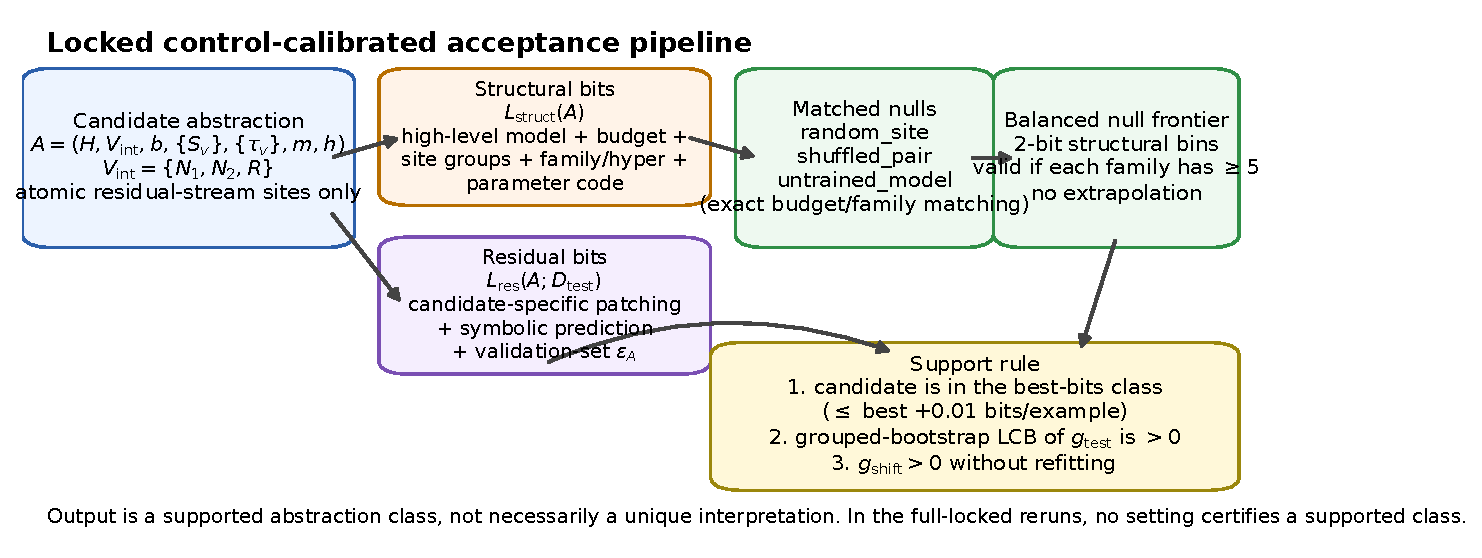
\includegraphics[width=\textwidth]{method_overview.pdf}
  \caption{\textbf{Locked acceptance pipeline.} Each candidate abstraction is a structured object over a fixed high-level model library, atomic residual-stream site groups, and a fixed readout family/hyperparameter grid. Candidates are scored by structural bits plus held-out residual bits from candidate-specific patching and symbolic prediction. Acceptance is not based on fit alone: a candidate must fall in a valid structural bin of the balanced matched-null frontier, lie in the best-bits class, have a positive grouped-bootstrap lower bound on the held-out test gap, and retain a positive shift gap without refitting. In the final full-scope reruns, no setting satisfies all of these conditions for any abstraction class.}
  \label{fig:method}
\end{figure*}

\paragraph{Candidate family.}
A candidate abstraction is
\[
A=(H,V_{\mathrm{int}},b,\{S_v\}_{v\in V_{\mathrm{int}}},\{\tau_v\}_{v\in V_{\mathrm{int}}},m,h),
\]
where $V_{\mathrm{int}}=\{N_1,N_2,R\}$, $H$ is one of four hand-written high-level models, $b$ is the site budget, each $S_v$ is a disjoint set of atomic residual-stream sites, and $(m,h)$ chooses a readout family and hyperparameter. The locked candidate pool contains four high-level models, three site budgets $b\in\{1,2,4\}$, and ten map-family/hyperparameter cells: one dense linear cell, three sparse-linear cells, three low-rank cells, and three one-hidden-layer ReLU cells, for $4\times 3\times 10=120$ candidate cells per setting before logged unevaluable cases.

\paragraph{Structural and residual code lengths.}
The primary score is
\[
\Ltot(A)=\Lstruct(A)+\Lres(A;D_{\mathrm{test}}).
\]
$\Lstruct$ charges the full explanatory object: high-level model ID, budget, site groups, map family and hyperparameter, and a BIC-style parameter code. $\Lres$ is computed on held-out interventions from a symmetric noise model whose error rate parameter is estimated on the validation split only. In S2 and S3 the observed output alphabet is closed with an \texttt{OTHER} class for patched outputs outside the locked name vocabulary; symbolic predictions are \emph{not} projected to \texttt{OTHER}.

\paragraph{Matched nulls and frontier.}
Candidates are not accepted by code length alone. For each structural bin, we build a matched null pool using three locked null families: \texttt{random\_site}, \texttt{shuffled\_pair}, and \texttt{untrained\_model} when available. Matching is exact on high-level model, site budget, map family/hyperparameter cell, optimizer logic, proposal budget, and splits. Structural bins have width 2 bits. A bin is valid only if each null family contributes at least five records. The balanced frontier value is the empirical 5th percentile of the matched null residual bits after balancing family counts, followed by an isotonic lower envelope. There is no extrapolation outside valid bins.

\paragraph{Acceptance rule.}
A candidate is supported only if all of the following hold simultaneously:
\begin{enumerate}[leftmargin=1.5em]
\item it lies in the \emph{best-bits class} $\Bbest$, i.e.\ within 0.01 bits/example of the best overall candidate in the setting;
\item its one-sided grouped-bootstrap lower confidence bound on the held-out test gap
\[
\gtest = \mathrm{frontier}_{\mathrm{test}}-\Lres(A;D_{\mathrm{test}})
\]
is positive;
\item its shift gap
\[
\gshift = \mathrm{frontier}_{\mathrm{shift}}-\Lres(A;D_{\mathrm{shift}})
\]
is positive without refitting.
\end{enumerate}
The output is a supported abstraction class rather than a unique interpretation.

\paragraph{Primary and robustness codebooks.}
The primary codebook uses the BIC-style parameter term from the method specification. The robustness analysis rewrites only the parameter code term using a quantized parameter code while leaving candidate search, null construction, frontier validity, and support logic unchanged.

\paragraph{Why this is a stringent test.}
The criterion intentionally couples compactness, null calibration, and out-of-distribution retention into a single acceptance decision. Any supported class would therefore be hard to dismiss as a flexible readout artifact. The downside is equally important: failure can arise either because matched nulls remain competitive or because support eligibility itself becomes geometrically narrow. One purpose of the paper is to disentangle those regimes empirically.

\section{Experimental settings and full-scope reruns}

All empirical claims in this paper are based on the final full-scope reruns and their audited summaries. Earlier reduced-scope pilots are excluded from the paper-level evidence base.

\paragraph{S1: planted symbolic/state generator.}
S1 is a deterministic residual-sequence model with an eight-symbol vocabulary and family-invariant relay sites for $(N_1,N_2,R)$ plus family-dependent nuisance structure. The planted oracle abstraction is
\[
\Astar=(H_{\texttt{true\_other}},\{N_1,N_2,R\},2,\{S^{\star}_v\},\texttt{linear\_dense},\texttt{default\_dense}),
\]
with exact planted site groups fixed by the generator. S1 contains 2,912 tuples split into canonical train/validation/test and a no-refit shift family.

\paragraph{S2: miniature learned IOI transformer.}
S2 is a locked two-layer decoder-only transformer (4 heads, $d_{\text{model}}=128$, $d_{\text{MLP}}=512$) trained from scratch on canonical-family next-token prediction with a four-name word-level vocabulary. The training artifact reaches canonical training accuracy 1.0. S2 contains 240 tuples.

\paragraph{S3: GPT-2-small IOI.}
S3 uses GPT-2-small \citep{radford2019language} with tokenizer-validated single-token names and the same canonical/shift IOI template family. S3 contains 72 tuples.

\paragraph{Configured versus realized coverage.}
The configured candidate family is identical across settings: 120 cells before logged unevaluable cases. S1 realizes all 120 cells. S2 realizes 116 cells and logs 4 unevaluable cells, still accounting for the full grid. S3 realizes 92 cells and logs 28 unevaluable cells, concentrated at $b=4$. This distinction is central to interpretation: full configuration coverage is necessary for the paper's negative claim, while realized coverage determines how broadly that claim should be read.

\section{Results}

\begin{table*}[t]
\caption{\textbf{Main full-scope results.} ``Closest frontier-defined'' denotes the frontier-defined candidate with smallest test total bits/example. $\Delta$ is its gap in test bits/example to the global best candidate. In every setting, the best-bits class contains exactly one candidate, and that candidate is frontier-ineligible.}
\label{tab:main}
\centering
\footnotesize
\begin{tabular}{lrrrrrrr}
\toprule
Setting & Cells & Valid bins & Best cand. & $\Delta$ to closest & $g_{\text{test}}$ & $g_{\text{shift}}$ & Supported \\
 & (rec./unev.) & (test/shift) & frontier? & frontier-defined &  &  & classes \\
\midrule
S1 planted & 120/0 & 3/3 & No & 2.008 & 0.000 & 0.000 & 0 \\
S2 mini-IOI & 116/4 & 3/3 & No & 0.066 & -0.155 & -15.582 & 0 \\
S3 GPT-2 IOI & 92/28 & 2/2 & No & 0.198 & -2.340 & -37.016 & 0 \\
\bottomrule
\end{tabular}

\end{table*}

\paragraph{No supported abstraction class is certified.}
Table~\ref{tab:main} summarizes the full-scope reruns. The frontier is not empty: S1 and S2 each have three valid bins on both test and shift, and S3 has two. Nevertheless, no setting certifies a supported abstraction class under the primary codebook, and the support count remains zero under the quantized robustness codebook as well.

\paragraph{Support failure has two regimes.}
The first regime is \emph{eligibility failure}. In all three settings the global best candidate lies outside the valid frontier domain. Because the best-bits class $\Bbest$ contains exactly one candidate in each setting, that candidate is ineligible for support by construction. The closest frontier-defined candidate therefore starts outside the acceptance gate.

The second regime is \emph{null-gap failure}. This is especially clear in the learned settings. In S2 the closest frontier-defined candidate has $\gtest=-0.155$ and $\gshift=-15.58$. In S3 the corresponding gaps are $\gtest=-2.34$ and $\gshift=-37.02$. So even if those candidates had entered $\Bbest$, they still would not have been supported.

\paragraph{The planted oracle still fails.}
The strongest S1 result is also negative. The exact planted oracle $\Astar$ is frontier-defined on both test and shift, yet still satisfies
\[
\gtest = 0,\qquad \gshift = 0,
\]
with grouped-bootstrap lower bound equal to zero. The criterion therefore does not recover the planted true abstraction over matched nulls in S1. This sharpens the interpretation of the negative result: the failure is not only about discovered candidates, but also about the behavior of the criterion on a hand-specified target abstraction.

\begin{figure*}[t]
  \centering
  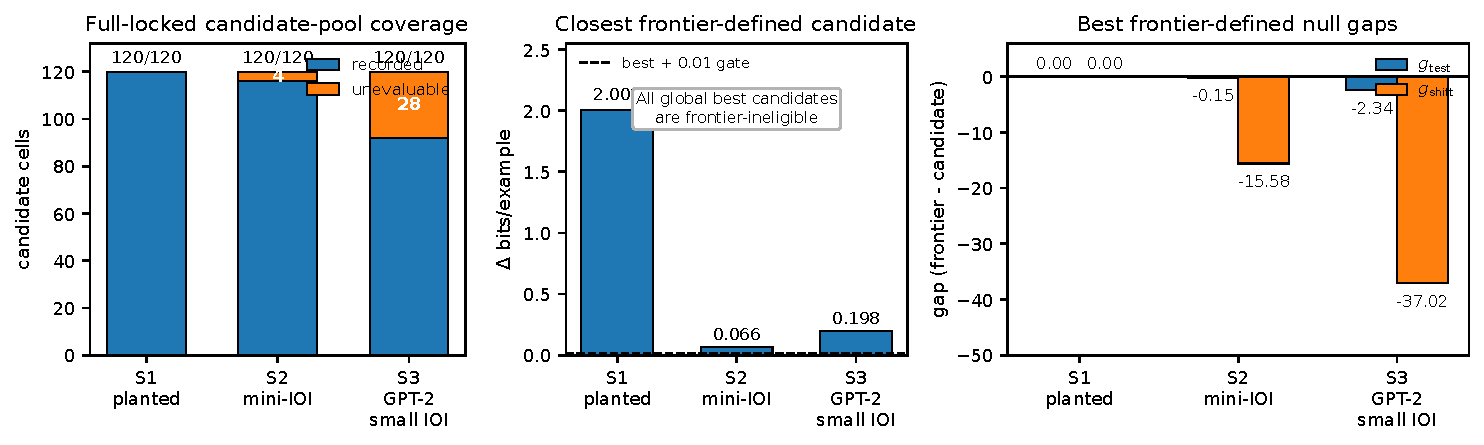
\includegraphics[width=\textwidth]{summary_panels.pdf}
  \caption{\textbf{Cross-setting summary from the full-scope reruns.} \textbf{Left:} recorded versus logged-unevaluable candidate cells, out of the locked 120-cell pool per setting. \textbf{Middle:} gap in test bits/example between the global best candidate and the closest frontier-defined candidate; the dashed line marks the locked best-plus-0.01 gate. \textbf{Right:} held-out test and shift null gaps for the closest frontier-defined candidate. The S1 planted oracle $\Astar$ also has $\gtest=0$ and $\gshift=0$. The full-scope negative result is therefore not just a search-slice artifact: S2 and S3 already fail on negative null gaps, while S1 exposes a frontier tie at zero.}
  \label{fig:summary}
\end{figure*}

\subsection{Why the full-scope reruns change the paper}

The negative result matters scientifically only because the full-scope reruns repair the earlier reduced-scope evidence problem. The configured candidate family is fully restored in all settings, and every missing realized cell is explicitly logged rather than silently omitted. This means the conclusion is no longer ``nothing survived a search slice,'' but ``nothing survived the locked family we set out to test.''

The reruns also show that the conclusion is not a fragile scoring artifact. Under the quantized robustness codebook, the best candidate identity is unchanged in all three settings and the support count stays at zero. The result is therefore stable to a meaningful rewrite of the parameter code term, even though it remains sensitive to the broader geometry of frontier validity and best-bits eligibility.

\subsection{Coverage and breadth of interpretation}

Full configuration coverage does not imply uniform realized coverage. S3 still contains 28 unevaluable cells, concentrated at $b=4$ and spread across all nontrivial readout families. This weakens breadth of interpretation at high complexity. At the same time, the core no-support result does not depend only on those missing cells, because the decisive failures already occur inside realized lower-complexity frontier bins.

\section{Implications for evidence standards}

The paper is most valuable if it yields reusable lessons for future acceptance criteria rather than stopping at ``no support found.'' We highlight three.

\paragraph{Control calibration is necessary but insufficient.}
Null calibration changes decisions in every setting. That is a positive methodological result: the criterion is not equivalent to choosing the minimum-code-length candidate and narrating it afterwards. But calibration alone does not produce certification. A future standard must therefore preserve matched controls while also making it plausible that good candidates can enter the support region at all.

\paragraph{Eligibility geometry must be reported separately from null-gap failure.}
The strongest interpretive caveat is geometric: the global best candidate is frontier-ineligible in all three settings, and the closest frontier-defined candidate lies outside the locked best-bits class. A paper that reported only ``no support'' would obscure whether failure came from competitive nulls or from the shape of the support domain. Our full-scope results suggest that these should be separated explicitly in future work. In S2 and S3 the negative result survives that separation because the closest frontier-defined candidates are already negative on both test and shift. In S1 the distinction is more consequential because the oracle and closest frontier-defined candidates tie the frontier at zero.

\paragraph{Configured-versus-realized candidate-pool accounting is part of the claim.}
The earlier reduced-scope package and the final full-scope reruns lead to very different evidentiary interpretations even though both ended with zero supported classes. This is not a bookkeeping detail. When support depends on matched null coverage and frontier validity, omissions and unevaluable cells alter what kinds of candidates can even be certified. Future mechanistic-interpretability evaluations should therefore treat candidate-pool accounting as first-class evidence.

\paragraph{Planted recovery should be checked directly.}
It would have been easy to summarize S1 as merely another no-support setting. The oracle evaluation shows something sharper: the exact planted abstraction does not beat the matched frontier and ties it at zero on both test and shift. That kind of direct planted check is more informative than inferring planted failure from aggregate search results.

\section{Related work}

Our starting point is the causal-abstraction program in mechanistic interpretability \citep{geiger2023causal}, especially distributed alignments between interpretable variables and neural representations \citep{geiger2024das}. The present paper asks a different question. Rather than proposing a new alignment method or a new abstraction-discovery routine, we ask whether a fully locked acceptance rule can serve as an evidence standard for top-down claims.

The work also connects to a broader line of warnings about evidentiary fragility. Control tasks for probes showed that apparently strong readouts can succeed for the wrong reasons unless matched controls are built into the methodology \citep{hewitt2019designing}. Subspace-patching results similarly highlight how intervention-based evidence can mislead when representation structure is under-constrained \citep{makelov2023subspace}. Our criterion internalizes those concerns by demanding matched null comparisons and held-out shift retention; the paper's contribution is to show that even this stronger protocol can still fail to certify.

Finally, S2 and S3 sit on standard transformer backbones \citep{vaswani2017attention,radford2019language}, while S1 is planted specifically to provide a direct oracle target. We intentionally keep the setting family narrow and auditable rather than broadening into a benchmark sweep. The contribution is therefore not benchmark breadth, but a sharply specified failure record for one candidate acceptance family.

\section{Limitations}

This paper has four important limitations.

First, it is a result about a \emph{locked family} of abstractions, nulls, and support rules, not about all possible abstraction families or all possible acceptance criteria.

Second, support failure is materially shaped by frontier-validity geometry. The global best candidate is frontier-ineligible in every setting, so the support rule's best-plus-0.01 gate is an important part of the story rather than an incidental detail.

Third, S3 retains many logged unevaluable high-complexity cells. The full-scope rerun makes those missing cells visible, but they still reduce the breadth of realized high-complexity evidence.

Fourth, the negative result is stronger in S2 and S3 than in S1. In the learned settings, the closest frontier-defined candidates have strictly negative test and shift gaps. In S1, by contrast, the most informative failure mode is a tie at zero, including for the planted oracle.

\section{Conclusion}

We evaluated a locked control-calibrated minimum-description criterion for top-down causal abstractions across three settings and found no supported abstraction class under either the primary or quantized robustness codebook. Because the paper is anchored to full-scope reruns rather than reduced pilots, this is a substantive negative result for the configured criterion family rather than a search-slice accident. The broader lesson is not that mechanistic interpretability is impossible, but that a credible acceptance standard must do more than combine compression with controls: it must also make frontier eligibility legible, report realized coverage explicitly, and demonstrate that planted targets can clear the same standard. In that sense, the criterion fails productively. It does not yet certify the abstractions we would want, but it clarifies what a better evidence standard must confront.

\bibliographystyle{plainnat}
\bibliography{refs}

\appendix

\section{Setting-specific failure summary}

The full-scope reruns reveal three distinct setting-level summaries.

\begin{itemize}[leftmargin=1.5em]
\item \textbf{S1 planted:} the global best candidate is frontier-ineligible, the closest frontier-defined searched candidate lies outside the best-bits class, and the exact planted oracle satisfies $\gtest=0$ and $\gshift=0$. The dominant failure mode is therefore a frontier tie at zero rather than a strongly negative gap.
\item \textbf{S2 mini-IOI:} the global best candidate is frontier-ineligible, the closest frontier-defined candidate lies outside the best-bits class, and that candidate is already negative on both test and shift. This is a stronger failure than mere eligibility geometry.
\item \textbf{S3 GPT-2 IOI:} the global best candidate is again frontier-ineligible, the closest frontier-defined candidate is already negative on both test and shift, and the frontier is sparsest because many $b=4$ cells are unevaluable. The learned failure signal is therefore accompanied by the weakest realized high-complexity coverage.
\end{itemize}

\section{Unevaluable cells by map family}

Table~\ref{tab:unevaluable} shows where logged unevaluable cells arise in the full-scope reruns. The main concentration is S3 at $b=4$.

\begin{table}[h]
\caption{\textbf{Unevaluable cells by map family.} Counts are over the locked 120-cell pool in each setting.}
\label{tab:unevaluable}
\centering
\small
\begin{tabular}{lrrrr}
\toprule
Setting & Dense & Low-rank & Sparse L1 & MLP1 ReLU \\
\midrule
S1 planted & 0 & 0 & 0 & 0 \\
S2 mini-IOI & 0 & 4 & 0 & 0 \\
S3 GPT-2 IOI & 4 & 8 & 8 & 8 \\
\bottomrule
\end{tabular}

\end{table}

\end{document}
